%Chapter 3 - Bringing open-source 8-bit projects to the market: challenges
%What are the challenges and pitfalls that face productising open-source retro computer projects?

\chapter{Bringing open-source 8-bit projects to the market: Case studies of similar projects and the challenges they faced}
\label{Chapter3}
By considering other similar projects and and highlighting the challenges they faced it is hoped that the MEGA65 project can avoid unnecessary delays and costs in the productisation process. This chapter outlines challenges that where faced by the teams behind the Spectrum Vega, Spectrum Vega+, Spectrum Next, Raspberry Pi, Arduino, C64DTV and C64Mini. These challenges where uncovered during case studies into these projects. This chapter also strives to highlight methods and activities used by the projects studied, that will help ensure the success of the MEGA65 project. 

%----------------------------------------------------------------------------------------
%----------------------------------------------------------------------------------------
\section{Open-source case studies}
The Arduino and Raspberry Pi where both studied because of their open-source nature, success and because both are relatively simple computers (in the general sense). These project share enough characteristics with the MEGA65 that some useful information was obtainable from these studies.

\subsection{Arduino}

\textbf{What is it?}\\
Arduino is a company which designs, produces and sells the Arduino range of single-board microcontrollers as seen in figure \ref{ArduinoUno3}, which are mostly 8-bit machines with 32-bit machines being introduced later. The Arduino company has released all the hardware designs as open-source under a Creative Commons licence. The associated IDE (Integrated Development environment) software is also open-source and Arduino also encourage and facilitate a community of hobbyist, open-source enthusiasts and professionals 
\cite{133}. \\

\textbf{When was it produced?}\\
The first Arduino board was designed and made available to students at the Interaction Design Institute Ivrea (IDII) in Italy in 2005. As word spread, the board quickly became popular outside of the class and Arduino boards remains hugely popular today 
\cite{RN103}.\\

\textbf{Why was it produced?}\\
It was used to help teach the students at IDII, interactive design (also known as physical computing). Massimo Banzi, a co-founder of Arduino, was using another commercially available microcontroller (the BASIC Stamp) to teach the class prior to the Arduino board being created (and its inspiration, Wiring) but it didn't meet his needs for teaching and it was too expensive for the students. Banzi decided to design his own microcontroller as associated IDE. Banzi drew heavy inspiration from another very similar project, Wiring, that was also in development at IDII before and during the creation of the first Arduino board. Wiring in turn built on another related project, Processing, which provided the starting point for the IDE used in Wiring. \\


\begin{figure} \begin{center}
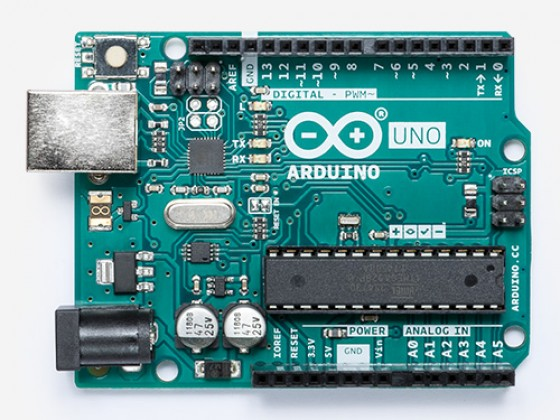
\includegraphics[width=.3\linewidth]{pics/Arduino_uno_3} 
\end{center} 
\caption{Arduino Uno Rev 3\\ \textit{\small{Picture from \url{https://store.arduino.cc/usa/}}}}
\label{ArduinoUno3}
\end{figure} 

\textbf{Challenges faced during productisation}\\
The biggest challenge for the Arduino company, in my opinion, was simultaneously making a profit for the company while being open-source with their products and allowing anyone to manufacture and sell them. Arduino handled this very successfully, with both the designs still being open-source and the company (Arduino LLC) still trading and appears to be reasonably profitable but as it is a private company it doesn't need to publish earnings. The original decision to make the designs open-source, according to Banzi 
\cite{RN111} \cite{RN103}, stemmed from the realisation that IDII was running out of money and would shut within a few years, potential endangering the Arduino project. Hernando Barragán, the creator of Wiring, claims Banzi and co. didn't have a choice but to make it open-source. As Arduino used work from Wiring and Processing and both where open-source and required any derivative to also be open-source 
\cite{RN110}. 
The Arduino team partnered with a manufacturer and got the first boards produced and sold for a small profit. Arduino found that as they were the first to market (with good reason) that they still sold a lot due to lack of competition, which was a possibility considering the open-source nature of the project. But when cheaper copies started being manufactured in Taiwan and China, this initially had the effect of increasing the sales through Arduino, even though there where cheaper versions available. Arduino put this down to the competition being of a lesser quality at that time 
\cite{RN113}. Arduino also charge a fee if other producers wanted to use the "Arduino" name. As the market matured, Arduino expected other producers and manufactures to be able to produce the Arduino boards at a cheaper price and of similar quality, which has happened. The Arduino company now focuses more on selling their expertise as the inventors, consultancy work, enabling the Arduino community and designing and selling Arduino accessories, such as 'shields', plug in devices that add extra functionality to the Arduino range 
\cite{RN113}.

The other big challenge Arduino faced was from legal challenges around ownership of the Arduino Trademark. In 2009, after the initial success of the Arduino boards, the co-founders decided they needed to create a company to hold all the trademarks and created Arduino LLC in the USA, as well as trademarking the name Arduino in the USA. It was decided to focus on the USA first, but one of the team members that was working on the production of the existing Arduino boards, separately registered the Arduino trademark in Italy without telling the rest of the Arduino team until 2014. In 2014, the company which held the Italian trademark and manufactured Arduino boards, Smart Projects, hired a new CEO. Smart Projects then changed its name to Arduino SRL and stopped paying Arduino LLC royalties for using the Arduino name 
\cite{RN115}. What followed was a drawn-out legal and community battle for a couple of years. In October 2016 the two parties announced an agreement to join forces and cooperate moving forward
\cite{RN116}. The schism seems to have come from two different parts of the initial group wanting to take the company in different directions, the production team wanting to keep production in Italy and the others wanting to expand into USA and China and let many other manufactures in. \\

\textbf{Relevant useful lessons gleamed from the study}\\
Open source hardware can make a profit in the short term by being first to market.
Open source businesses can generate profit in other ways including: consultation or selling expertise of the product, licence fees for use of trademark such as Arduino did with their name as well as designing and producing accessories.
It is extremely important to keep control of trademarks and other intellectual property (IP). It is recommended that MEGA65 seek guidance from an IP expert, in the hope of avoiding Arduino's trademark problems. 
Open-source projects encourage others to participate simple by being open, this in turn creates a community of people, these open-source communities seem to naturally converge around the original creator/s. the original creator of the Linux kernel, Linus Torvalds and the communities around Arduino and Raspberry Pi are other examples of this. The original creator/s, by being the focal point, should generally be well informed on what the community is doing, this can be leveraged by hosting community-oriented services, such as forums to share ideas and knowledge which in turn should increase the popularity of the product. \\

\subsection{Raspberry Pi}


\textbf{What is it?}\\
A cheap, open-source, single-board computer which runs a version of the Linux operating system shown in figure \ref{Raspberry_Pi}. The first version had a 32-bit processor with later version including a 64-bit processor, it's worth noting the processor chip itself is not open-source
\cite{RN99}.\\

\textbf{When was it produced?}\\
The Raspberry Pi vesion 1 Model B was first sold in February, 2012 for \$35, with Model A coming out soon after for \$25 \cite{RN100}.\\

\textbf{Why was it produced?}\\
In 2006, Eben Upton, who grew up using a BBC Micro (from the early home computer era), had a desire to help kids learn computer science and related topics. He compared the BBC Micro on which he learned, which booted up straight into a BASIC command prompt, to modern devices children have access to, such as a tablet. He lamented that a child with a tablet is so far removed from the inner workings of the device that learning computer programming and related skills is a lot more difficult \cite{RN97}. To achieve his goal of helping kids learn about computers, Upton decided to make a small, cheap computer which would hopefully encourage kids to play and learn, as he did with the BBC Micro. Upton and several others formed a charity in 2009 with the purpose of advancing this agenda, called The Raspberry Pi Foundation. It wasn't until a few years later that Upton found a suitable chip for the Raspberry Pi. While working for Broadcom on the design team for the BCM2835 chip, Upton realised the BCM2835 would be perfect for the Raspberry Pi computer he had envisaged
\cite{RN97}.\\

\begin{figure} \begin{center}
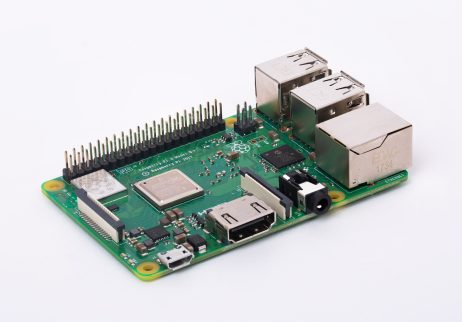
\includegraphics[width=.3\linewidth]{pics/Raspberry_Pi_3B+} 
\end{center} 
\caption{Raspberry Pi 3 Model B+\\ \textit{\small{Picture from \url{https://www.raspberrypi.org/products/}}}}
\label{Raspberry_Pi}
\end{figure} 

\textbf{Challenges faced during productisation}\\
The Raspberry Pi productisation process seems to have avoided most major problems, how much of this can be attributed to Upton waiting for a chip that suited the project is hard to decipher, but it most definitely helped. Whether waiting for a suitable chip is a challenge or not depends on the project.
The Raspberry team announced a release date before the final product was ready, this added a lot of pressure during that window to meet their self imposed deadline, this added stress to the creators but may have helped push the project along at a faster pace than without the deadline \cite{RN97}. 
The Raspberry Pi was delayed in the first production run due to compliance laws in Europe around electronic interference compliance. The Raspberry Pi needed to be tested for electronic interference but the creators didn't realise this until it was too late to avoid delays \cite{RN98}.  

\textbf{Relevant useful lessons gleamed from the study}\\
Open source hardware can be incredibly popular. 
Check relevant laws and seek expert advice early as possible to avoid delays in production.\\

\section{Retro revival project case studies}
These case studies look at a group of products that are inspired by 8-bit computers from the home computer era mentioned in \ref{sec: Early home computer era}. Two of the biggest names from that time, Spectrum, popular in Britain and Commodore, popular in the USA are both reproduced in modern revival projects. These projects are similar to the MEGA65 project and as such are studied in the hope of increasing the chance of the MEGA65 being successful. 

\subsection{Sinclair ZX Spectrum Vega}

\textbf{What is it?}\\
The Sinclair ZX Spectrum Vega is a game console inspired by the ZX Spectrum (another hugely popular home computer from the early home computer era \ref{sec: Early home computer era} which was released in the United Kingdoms in 1982 by Sinclair Research. The ZX Spectrum Vega comes preloaded with 1000 games, most of which where written for the original ZX Spectrum. It swaps the full keyboard of the original for a directional thumb pad and 9 rubber buttons as shown in figure \ref{Spectrum_Vega}. It has the endorsement of Sir Clive Sinclair, the founder of Sinclair Research. The Vega was created by Retro Computers and uses a hardware design created for the project and has a microcontroller at its core and custom-built software to allow it to play all games written for the ZX Spectrum \cite{RN119}.

\textbf{When was it produced?}\\
The Vega was released in April 2015, following a successful crowd-funding campaign on Indiegogo, a crowd-funding service. It cost 100 pounds at launch but is no longer produced or sold by Retro Computers as they have run into financial and legal troubles relating to another product, the Vega+ and was recently wound up 
\cite{RN120}.  

\textbf{Why was it produced?}\\
The Sinclair ZX Spectrum Vega was a commercial endeavour. 

\begin{figure} \begin{center}
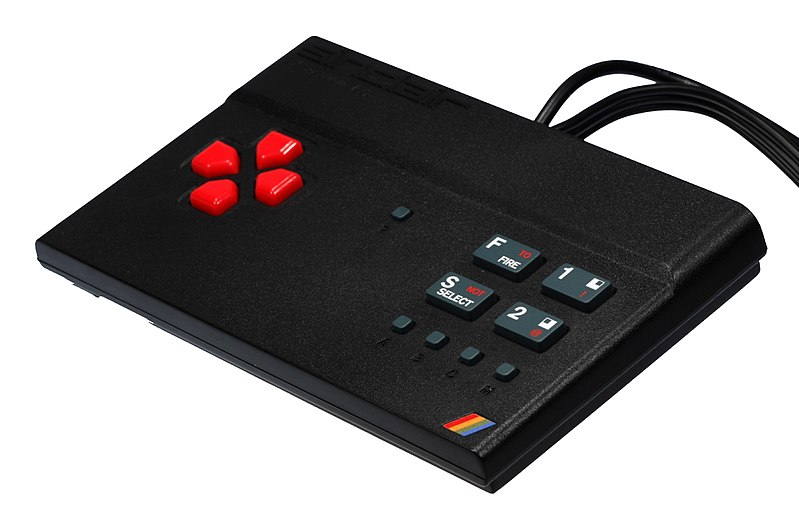
\includegraphics[width=.3\linewidth]{pics/Spectrum_Vega} 
\end{center} 
\caption{Sinclair ZX Spectrum Vega, a game console with 1000 preloaded games inspired by the ZX Spectrum from 1982. \\ \textit{\small{Picture courtesy of Marco Tangerino}}}
\label{Spectrum_Vega}
\end{figure} 

\textbf{Challenges faced during productisation}\\
The Indiegogo campaign was successful, raising 149\% of the funding goal 
\cite{RN119}. 
Retro Computers launched a crowd-funding campaign offering a product to backers which wasn't complete yet, since this campaign, there has been a successful legal challenge that states that this type of agreement is a sales contract and such they are legally obliged to deliver the product regardless of problems that could arise before the product is complete 
\cite{RN122}. This ruling came from legal action against the Indiegogo crowd-funding campaign for next iteration from Retro Computers the Sinclair ZX Spectrum Vega Plus console. So by offering a product to backers in a crowd-funding campaign, Retro Computers exposed themselves to extra risk and it may have been better to word the crowd funding campaign differently to avoid this or just not offer the product to backers at all but rather sell it to them cheaper once it is finished (if it gets finished).

\textbf{Relevant useful lessons gleamed from the study}\\
Crowd-funding campaigns can be useful to raise capital but offering a as-yet unfinished product to backers exposes the campaign founders to an amount of risk in that they legally have to deliver the product and there may be unforeseen costs and challenges in producing it.

\subsection{Spectrum Vega+}

Sinclair ZX Spectrum Vega mention earlier. It is, like it predecessor, inspired by the Sinclair ZX Spectrum and also has the endorsement of Sir Clive Sinclair, although it is reported he has very little to do with the actual running of Sinclair Research 
\cite{RN123}. The Vega Plus is a hand-held console with its own screen and internal battery as well as the ability to output its display to a TV, although this feature couldn't be made to work in a review of the Vega Plus 
\cite{RN117}.

\textbf{When was it produced?}\\
In July 2018, Retro Computers sent out a number of Vega Plus consoles to backers. No other Vega Plus consoles have been produced.

\textbf{Why was it produced?}\\
Like its predecessor the Vega Plus was a commercial endeavour. 

\begin{figure} \begin{center}
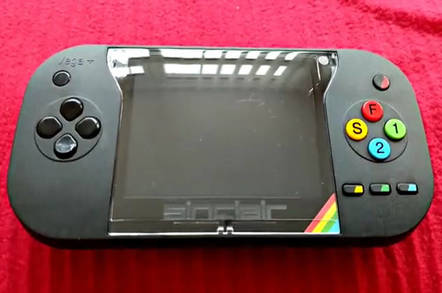
\includegraphics[width=.3\linewidth]{pics/Spectrum_vega_plus} 
\end{center} 
\caption{Sinclair ZX Spectrum Vega Plus console, the poorly received culmination of a tumultuous crowd-funding campaign  \\ \textit{\small{Picture courtesy of Craig Wootton}}}
\label{Spectrum_Vega_Plus}
\end{figure} 

\textbf{What is it?}\\
A iteration of the 

\textbf{Challenges faced during productisation}\\
The Vega Plus crowd-funding campaign and subsequent unkept promises of delivery from Retro Computers has been reported as one of the worst crowd-funding disaster stories ever. With the Indiegogo campaign raising 366\% of the funding goal, over half a million pounds (over \$900,000 AUD), following on from a successful campaign with proven results and the backing and involvement of home computer era luminaries Sir Clive Sinclair and designer Rick Dickinson as well as a working prototype and completed designs for the Vega Plus as well as the expertise within Retro Computers to finish the product, it was be fair to give the project a fair chance of success in finishing the Vega Plus and delivering them to backers. What actually occurred can not be called successful by any metric and it is amazing to compare to very poorly received results with the potential at the beginning of the campaign.  

The first and biggest challenge faced was that very early into the campaign, two of the directors of Retro Computers resigned including the CTO Chris Smith who was the designer of the Vega Plus prototype and held the rights to it, which he took with him when leaving the company. This left Retro Computers having to start from scratch with the hardware design and firmware for the Vega Plus after already promising over 4000 backers they would deliver a Vega plus. This in turn lead to delays. Retro Computers made many failed promises of delivery to the backers during this time, cause much angry from the backers. Several legal actions followed, most notable a backer took Retro Computers to court claiming they broke a contract of sale with him over the Vega Plus. Interestingly Indiegogo's terms explicitly state that any rewards to backers are perks or gifts but the court ruled differently in part because the receipt to the backer for his pledge stated his order for a Vega Plus had been received and this formed a contract of sale between Retro Computers and the backer (not Indiegogo). Retro Computers now legally had to deliver the Vega Plus or refund the backers money, but reports from the times show Retro Computers was haemorrhaging money and didn't have a working prototype. Retro Computers then lost the rights to use the 1000 games that where included on the Vega, this was due to the license holders, Sky (Media?) withdrawing support due to the ongoing controversy surrounding the Vega Plus which was already well behind its delivery date with no progress to show. Retro Computers eventually managed to scrape together a barely functional console using a open-source spectrum emulator called FUSE (Free Spectrum Emulator) and a collection of 8? games all made by a single developer that was closely associated with Retro Computers and the Vega Plus project. Retro Computers claims they sent out 400 Vega Plus consoles to backers, with no word of when the rest are coming. One concerned backer did some investigating and found the number of consoles sent out to be closer to 50. Following this, Retro Computers was wound-up by an ex-director of Retro Computers, while functioning as the director of another company, claiming the Retro Computers owns them money. So as it stands Retro Computers is closed, no more Vega Plus (or indeed Vega) consoles are likely to be made and a large amount of money has gone missing with very little to show for it. There is ongoing legal actions against various directors of Retro Computers about these issues.

\textbf{Relevant useful lessons gleamed from the study}\\
Keep control of needed intellectual property needed for the project, form agreements with holders of IP for there use in the project before making any promises of delivery of product. Don't do anything to jeopardize any current contracts, such as Retro Computers did to lose the backing of Sky and thus the ability to include the games they had promised.
Be honest with backers and investors as to the state of the project, this is especially true for crowd-funding backers as these campaigns generally involve a large number of people.
Don't make claims or promises that cannot be kept in reasonable circumstances.
Crowd-funding campaigns offering products to backers can possible be seen to be a contract of sale between the backers and the campaign founders. This in turn forces the campaign founder to act according to the law regarding a contract of sale, including such things as refunds and guarantees of delivery.


\subsection{ZX Spectrum Next}

\textbf{What is it?}\\
The ZX Spectrum Next is a fully functional 8-bit computer that closely emulates the Sinclair ZX Spectrum from 1982. It achieves this by emulating the Spectrum in a FPGA board. The maker claim they will release the hardware design as open-source once it is complete. The case design is by Rick Dickinson the celebrated case designer of the original Spectrum series.

\textbf{When was it produced?}\\
It is currently under production. The Next is the focus of a Kickstarter crowd-funding campaign, which was launched in April 2017 and gave the original delivery date as January 2018. The campaign was well funded, raising £723,390 from over 3000 backers.

\textbf{Why was it produced?}\\
A commercial enterprise.

\begin{figure} \begin{center}
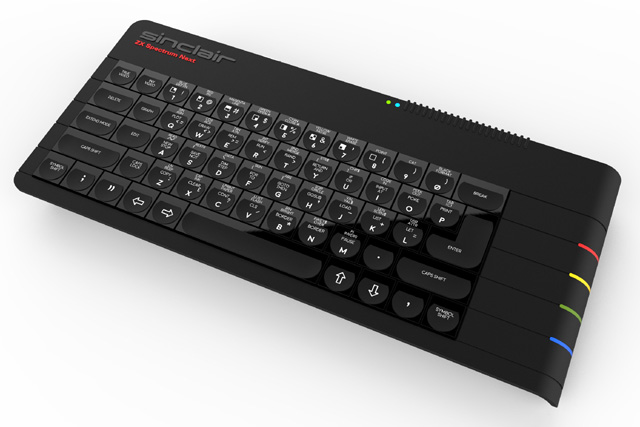
\includegraphics[width=.3\linewidth]{pics/spectrum_next} 
\end{center} 
\caption{ZX Spectrum Next, intended to be a fully functional iteration of the Sinclair ZX Spectrum. The makers claim it will be fully compatible with all software written for the original Spectrum \\ \textit{\small{Picture from \url {https://www.specnext.com/about/}}}}
\label{Spectrum_Next}
\end{figure} 

\textbf{Challenges faced during productisation}\\
The makers have had trouble with the mechanical function of the keyboard which has delayed production while they try to fix the issue. The last given expected delivery date was the 2nd quarter of 2019. There is also evidence the firmware the Next is running is still under development.

\textbf{Relevant useful lessons gleamed from the study}\\
As the project is not finished yet it is hard to gleam anything useful. Give plenty of time (if possible) to quality control and testing of the buttons and keys.

\subsection{C64 Mini}
\textbf{What is it?}\\
A mini form-factor game console inspired by the Commodore 64. It also is a fully functional Commodore 64 which can be control via a USB connected keyboard (not included). It has a non-functional keyboard and a functional joystick which connects to the console. The  console then connects to a TV to display in 720p resolution. It came pre-loaded with 64 game written for the Commodore 64, it also has the ability to load game ROMs from a USB flash stick. It was funded through a crowd-funding campaign on Indiegogo 
\cite{RN124} with the intention of making a full size version after the mini version. It's interesting to note that the resigned directors of Retro Computers (they company behind the unpopular Vega Plus campaign), Paul Andrews and Chris Smith (they resigned before the company went off the rails) are involved as well as Darren Melbourne who worked on the C64 DTV 
\cite{RN127}.

\textbf{When was it produced?}\\
Released in the first quarter of 2018.

\textbf{Why was it produced?}\\
To make money.

\begin{figure} \begin{center}
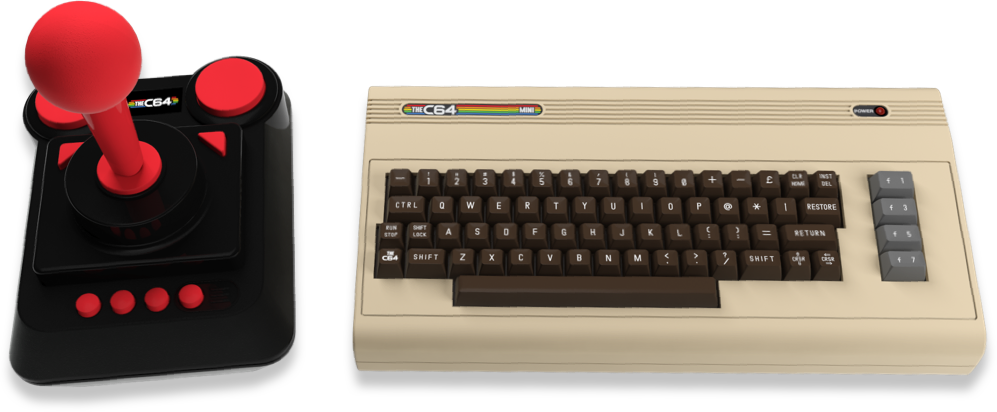
\includegraphics[width=.3\linewidth]{pics/C64_mini} 
\end{center} 
\caption{C64 mini\\ \textit{\small{Picture from \url {https://retrogames.biz/thec64-mini/}}}}
\label{C64_mini}
\end{figure}

\textbf{Challenges faced during productisation}\\
The crowd funding campaign did not meet the target goal of \$150,00 USD, reaching 67\% of the target or \$100,611 USD. Retro Games delayed their production schedule because of this, but ultimately they reached and agreement with an international distributor and manufacturer which allowed them to continue without seeking further funding
\cite{RN125}. This collaboration with the aforementioned partner also lead Retro Games to rethink their plans, they pivoted to focus on the C64 mini version entirely and get that complete first before moving to the full size version.

\textbf{Relevant useful lessons gleamed from the study}\\
Regular communication with backers is important for a successful crowd-funding campaign, this includes listening to them and responding to their concerns and queries. Paul Andrews and Chris Smith must have been aware there could be potential backlash over their involvement in the Vega Plus quagmire (they where both directors of Retro Computers when the Vega Plus campaign was launch but left a few months later). They remained honest (to the best of my knowledge) about the situation and who they where and probably of most importance, gave regular weekly updates to backers describing progress made and relevant news as well as progress pictures whenever possible. They also, on several occasions, publicly answered specific questions from backers, which would go a long way to alleviating fears and concerns from the backers about a repeat of the Vega Plus campaign.  


\subsection{C64 DTV}
\textbf{What is it?}\\
A single-chip Commodore 64 clone housed within a joystick, comes preloaded with 30 games. It was, unsurprisingly from the name, inspired by the Commodore 64. It features a FPGA at its core and has the possibility of after market modification due to exposed solder points on the board
\cite{RN126}. 

\textbf{When was it produced?}\\
First released in 2014 with version 1, which support only NTSC Broadcasting Television standard. Version 2 came out in 2015 with additional PAL support

\textbf{Why was it produced?}\\
A commercial endeavour. 

\begin{figure} \begin{center}
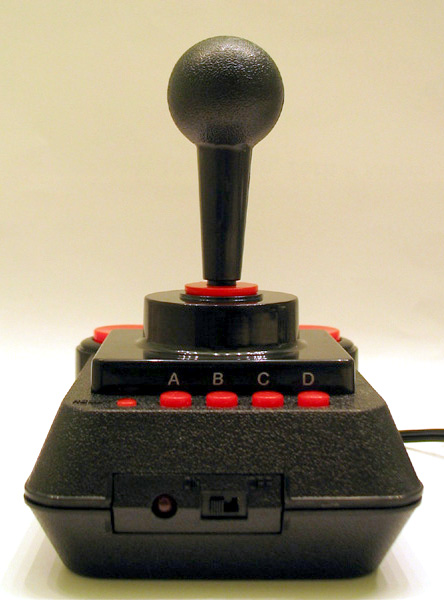
\includegraphics[width=.3\linewidth]{pics/C64_DTV} 
\end{center} 
\caption{C64 DTV or C64 Direct-to-Television \\ \textit{\small{Picture courtesy of Christian Wirth}}}
\label{C64_DTV}
\end{figure}

\textbf{Challenges faced during productisation}\\
The C64 DTV was derived from another similar product, the C-One. Jeri Ellsworth designed an enhanced version of the Commodore 64 as a way to teach herself about programming FPGAs. Ellsworth then partnered with Individual Computers to turn her FPGA design into a product, the C-One. Other manufactures and retailers saw potential in the C-One and asked if Elleworth would consider making a smaller version that would fit in a joystick and be designed to enable users to play Commodore 64 games easily. Unfortunately it seems very little was published about the process from turning the C-One into the C64 DTV or from earlier efforts to complete the C-One.


\textbf{Relevant useful lessons gleamed from the study}\\
Retro games can sell quite well, nostalgia is a powerful incentive.
Extra features included in the device can help boost sales, these can be features that are not normal available but the device can be hacked or modified by the user to make them available.